% TODO: port into host Overleaf template (https://www.overleaf.com/read/vjztpvrnbrdh)
\documentclass[10pt,twocolumn]{article}
\usepackage[a4paper,margin=1.7cm,columnsep=0.6cm]{geometry}
\usepackage{graphicx,booktabs,amsmath,amssymb,xcolor}
\usepackage[hidelinks]{hyperref}
\usepackage[compact]{titlesec}
\usepackage{enumitem}
\setlist{nosep,leftmargin=*}
\titlespacing*{\section}{0pt}{4pt}{2pt}
\titlespacing*{\subsection}{0pt}{3pt}{1pt}
\setlength{\parskip}{1pt}
\setlength{\textfloatsep}{6pt}
\newcommand{\todo}[1]{\textcolor{red}{[TODO: #1]}}
\newcommand{\dpq}{$\Delta$PQ}

\title{\vspace{-1.2cm}Solar Filament Instance Segmentation on GONG H$\alpha$:\\
a P2/stride-2 YOLO detector, crop refiner and agreement-calibrated keep rule}
\author{Team WeAreBatman: \todo{author names} \quad Repository:
\href{https://github.com/Amjath-s/kaggle-solar-filament-/tree/v84-final}{github.com/Amjath-s/kaggle-solar-filament- (branch v84-final)}}
\date{\vspace{-0.9cm}}

\begin{document}
\maketitle

\begin{abstract}
We segment solar filaments on $2048^2$ GONG H$\alpha$ images with a P2-augmented YOLO11s-seg detector,
4-flip consensus, a ResNet18 U-Net crop refiner and a learned keep rule that demotes masks a random
annotator is unlikely to have drawn. On 5-fold out-of-fold (OOF) validation over all 707 training files the
final pipeline reaches PQ \textbf{0.4590} (public LB 0.39). Human annotators agree with each other at only PQ
$\approx$0.34, and most residual error is annotator disagreement rather than mask quality. Nineteen further
pre-registered experiments (larger detectors, a second detector, Mask2Former alone and as a second opinion, a
whole-disk U-Net, agreement-only labels,
metric-aligned losses, fragment merging, a pixel-based quality head, per-instance thresholds) did not improve it
by more than +0.002.
\end{abstract}

\section{Task, metric and validation}
\textbf{Data.} 707 training files with 1154 annotator records and 8199 polygons (411 files have one record,
145 two, 151 three); 180 test images. \textbf{Metric.} Panoptic Quality with IoU$>$0.5 matching, where each
prediction set is matched separately against every annotator record and TP/FP/FN are pooled over all
(image, record) pairs. A filament drawn by $k$ of $n$ annotators and predicted with IoU $s$ thus earns
$k$ TP and $n-k$ FP, so predicting it pays only if roughly $k/n > \mathrm{PQ}/(2s)\approx0.31$: the target is
``would a random annotator draw this'', not ``is this a filament''. Our scorer reproduces the host
self-evaluation notebook exactly (identical TP/FP/FN on all 707 files).

\textbf{Validation protocol.} 5-fold OOF split by file (141--142 files per fold); every file is predicted by
detector, refiner and keep-rule models that never saw it (the refiner and the keep rule are refit per fold:
``leak-free'' refined OOF). Each experiment is \emph{pre-registered}: arms, metric, and a mechanical
CONTINUE/KILL gate are written and hashed (sha256) before any number exists. Comparisons use a paired
file-level bootstrap (2000 resamples) and report \dpq, 95\% CI, $P(\Delta>0)$ and per-fold signs. Typical gate:
pooled \dpq$\ge$+0.010 (screens) or $\ge$+0.005 (final bundle), $P\ge0.90$, $\ge$4/5 folds positive; KILL if
\dpq$<$+0.005. Seed/retraining noise is measured, not assumed (detector seed noise $-0.005$ on fold 0;
refiner retraining noise $\approx$0.0001). The public LB shows two decimals on $\sim$90 images and cannot
resolve the effects below, so it was not used for selection.

\section{Pipeline}
\textbf{(1) Detector: ``p2first'' YOLO11s-seg.} We add a P2 level to YOLO11s-seg (Upsample $\to$ Concat with
backbone P2 $\to$ C3k2[128]) and place it \emph{first} in the Segment head inputs [P2,P3,P4,P5]. Because
Ultralytics builds mask prototypes from the first input, this gives stride-2 prototypes (512$\times$512 at
1024 input) plus stride-4 detection, which matters for thin, small filaments. Init: COCO YOLO11s-seg with
head tensors re-indexed (509/639 tensors transfer). Training: single class, imgsz 1024, batch 4, 80 epochs at
mask\_ratio 2 then 20 epochs at mask\_ratio 1 (AdamW $10^{-4}$); one record = one training image. The
final detector is retrained on all 707 files.

\textbf{(2) 4-flip TTA and consensus.} Inference on identity, H, V and HV flips; masks are clustered across
views (anchor = highest score, IoU 0.5), cluster score = sum of view scores / 4. \textbf{(3) Pixel ownership.}
Score-ordered ownership makes instances pixel-disjoint (required by the host).

\textbf{(4) Crop refiner.} A ResNet18 U-Net on 256-px proposal-centred crops (4-flip TTA) re-predicts each mask
at full 2048 resolution, clamped to a 7$\times$7 dilation of its seed. It is trained on the detector's
\emph{own OOF proposals} in two stages: (A) 8 epochs on GT crops (lr $3\cdot10^{-4}$), (B) 12 epochs on
proposals matched to GT (IoU$\ge$0.3), 0.5 BCE + 0.5 Dice. V84 uses \emph{soft targets} in stage B: the target is the per-pixel mean, over the $R$ annotator records, of the GT mask each record matched to the
proposal (0 for records without a match), so the refiner learns agreement-weighted extent. Mask threshold $t=0.50$, detection cut $c=0.30$.

\textbf{(5) MIN200 + demote rule.} Masks below 200 px are dropped. A LightGBM regressor (28 features:
consensus and member scores, view support, ownership retention, refined-probability statistics, area, elongation, width, disk position, contrast, disk statistics,
neighbour and per-file counts) predicts for each kept mask $j$ the expected per-record matched quality
$\hat y_j\approx q_j s_j$, where $q_j$ is the fraction of records that match it and $s_j$ the mean matched IoU.
Since PQ $=\sum q s/(\text{TP}+\tfrac12\text{FP}+\tfrac12\text{FN})$, adding mask $j$ raises PQ iff
$q_j s_j > \mathrm{PQ}\cdot\tfrac12$; the optimal keep set is therefore a threshold on $\hat y$ at $\lambda/2$, with
$\lambda$ the fixed point $\lambda=\mathrm{PQ}(\{j:\hat y_j>\lambda/2\})$ found by Dinkelbach iteration
(converges in a few steps; $\lambda=0.4587$ on pooled cross-fitted OOF). Rule: keep $j$ iff $\hat y_j>\lambda/2$.
Only demotion is used (promoting masks below $c$ gave +0.0001). On OOF it removes 9.3\% of masks
(4686$\to$4248), on test 8.3\%.

\textbf{(6) Export.} Native 2048 masks, COCO RLE, validated (non-overlap, full decode) before writing.

\section{Results}
\begin{table}[t]\centering\small
\caption{5-fold OOF, 707 files, pooled per-record PQ. Baseline = V65 deployed path (p2first + r3 refiner,
$t$0.45/$c$0.30) with leak-free 5-fold refiner. Paired bootstrap vs baseline.}
\label{tab:main}
\setlength{\tabcolsep}{3pt}
\resizebox{\columnwidth}{!}{\begin{tabular}{lcccc}
\toprule
pipeline & PQ & SQ & TP/FP/FN & \dpq\ [95\% CI] \\
\midrule
V65 path (baseline) & 0.4539 & .685 & 5270/2444/2929 & -- \\
\textbf{V84 (final)} & \textbf{0.4590} & .688 & 5050/1881/3149 & \textbf{+0.0050} [+.0024,+.0077] \\
\midrule
only soft targets & 0.4550 & .685 & & +0.0011 [+.0001,+.0021] \\
only $t$0.50 & 0.4546 & .686 & & +0.0007 [$-$.0001,+.0015] \\
only MIN200 & 0.4560 & .685 & & +0.0021 [+.0014,+.0029] \\
only demote & 0.4569 & .687 & & +0.0030 [+.0007,+.0053] \\
V84 $-$ MIN200 & 0.4590 & .688 & & +0.0051 [+.0023,+.0077]\\
V84 $-$ demote & 0.4567 & .686 & & +0.0028 [+.0013,+.0044]\\
\bottomrule
\end{tabular}}
\end{table}

Table~\ref{tab:main} gives the final comparison. The V84 bundle gains \dpq\ = +0.0050, CI [+0.0024, +0.0077],
$P(\Delta>0)=0.9995$, positive on 5/5 folds (+.0057, +.0097, +.0028, +.0027, +.0045). It met its
pre-registered +0.005 bar by only 0.00004, so we expect $\approx$+0.005$\pm$0.003 on test, not a certain gain.
Single components sum to +0.0069; the bundle keeps 73\%. The demote rule is the largest marginal component and
makes MIN200 redundant (the bundle without MIN200 is +0.00002 better; MIN200 is kept as a harmless export
default). Both V65 and V84 score \textbf{0.39} on the public LB, which is consistent with a +0.005 effect
being below its two-decimal resolution.

Earlier milestones (direct detector, 707 files): baseline YOLO11s-seg 0.3856 $\to$ p2first 0.4060
(\dpq\ +0.0204 [+0.0151, +0.0256], 5/5 folds; small-object recall 0.411$\to$0.460). The crop refiner adds
$\approx$+0.04--0.06 PQ on top of any detector, mostly via SQ (0.657$\to$0.689).

\textbf{Negative results: the refiner absorbs detector gains.} Table~\ref{tab:neg} lists pre-registered
experiments that were killed by their gates. A recurring finding is that improvements that are clear on
the direct detector vanish after refinement: the refiner already fixes mask geometry, so detector gains
must come from \emph{instance selection}, not extent. From V76 on, every detector change had to pass a
refined-pipeline gate.

\begin{table}[t]\centering\small
\caption{Selected pre-registered negatives. Direct = detector only; refined = through the refiner. 141 held-out files (fold-0 screens or canonical
hold-out), except refiner variants and re-scorer (707-file 5-fold).}
\label{tab:neg}
\setlength{\tabcolsep}{2.5pt}
\resizebox{\columnwidth}{!}{\begin{tabular}{lll}
\toprule
change & direct \dpq & refined \dpq\ [95\% CI] \\
\midrule
imgsz 1280 & +0.0143 & $-$0.0029 [$-$.013,+.007] \\
thin labels ($-$1 px polygons) & +0.0272 & $-$0.0017 [$-$.010,+.007] \\
noisy student (unlab.\ GONG) & +0.0106 & +0.0007 [$-$.010,+.011] \\
label transfer $\pm$1/2/5 min & $-$.011/+.001/$-$.006 & not run (killed) \\
2-detector ensemble & +0.0063 & +0.0016 [$-$.006,+.009] \\
refiner: union targets & -- & $-$0.0195 [$-$.026,$-$.013] \\
refiner: quality-weighted & -- & $-$0.0000 [$-$.002,+.002] \\
refiner: crop512 / RN34 / dil15 & -- & +.0000 / +.0006 / +.0006 \\
learned re-scorer (agreement) & +0.0161 & $-$0.0099 [$-$.018,$-$.002] \\
\bottomrule
\end{tabular}}
\end{table}
Other closed lines: Mask R-CNN, Mask2Former, DenseCRF, BCE+Focal+Dice loss, YOLO11m, size-gated refiner
($-$0.014), 1-px erosion of refined masks ($-$0.024). Soft targets (+0.0019, fold 0) and the keep rule
(+0.0030, 707 files) failed their \emph{individual} gates and were only adopted as a re-registered bundle.

\begin{table}[t]\centering\small
\caption{Pre-registered experiments after V84, each against V84 on the same files. Scope: 707 = all files,
5-fold, full V84 path with the demote rule refit on the arm's own candidates (V84 0.4590); f0 = fold 0, 141 files,
refined path at cut 0.30 (V84 0.4555) or full path (0.4590) as pre-registered per experiment. Refiner seed
noise on fold 0 is $\pm$0.002.}
\label{tab:post}
\setlength{\tabcolsep}{2.5pt}
\resizebox{\columnwidth}{!}{\begin{tabular}{llc}
\toprule
change & scope & \dpq\ [95\% CI] \\
\midrule
pooled 3-detector candidates + learned selector & 707 & +0.0003 [$-$.003,+.004] \\
pixel ownership by refiner argmax (not score order) & 707 & $-$0.0021 [$-$.004,+.000] \\
SSL-initialised refiner (MIM / MoCo on GONG) & f0 & $-$0.0011 / $-$0.0027 \\
4-seed refiner ensemble & f0 & +0.0003 [$-$.004,+.004] \\
spine-first instances as extra candidates & 707 & +0.0011 [$-$.001,+.003] \\
detector fine-tuned on hardest annotators' style & f0 & $-$0.0138 (own subset) \\
refiner retrained on 1280-px proposals & f0 & $-$0.0010 \\
refiner with hard-negative crops + seed veto & f0 & $-$0.0020 \\
8-view (rot90 + flip) detector TTA & f0 & +0.0005 \\
YOLO11m + train-time flips & f0 & $-$0.0100 [$-$.023,+.001] \\
Mask R-CNN as gap filler (YOLO first) & f0 & $\pm$0.0001 \\
whole-disk ConvNeXt-T U-Net blended into crop prob. ($w$=0.5) & f0 & $-$0.0050 [$-$.011,+.001] \\
detector fine-tuned on annotator-agreed filaments only & f0 & $-$0.0190 [$-$.032,$-$.006] \\
refiner loss: Lov\'asz / + Skeleton Recall & f0 & $-$0.0018 / $-$0.0070 \\
merge collinear fragments (nested CV gap, angle) & 707 & $-$0.0002 \\
quality CNN on 5-ch crops, averaged with LightGBM & 707 & +0.0019 [+.0003,+.0035] \\
per-instance threshold maximising expected IoU & 707 & $-$0.0007 [$-$.002,+.001] \\
Mask2Former Swin-T: standalone / through our refiner & f0 & $-$0.095 / $-$0.120 \\
Mask2Former agreement as keep-rule features (nested CV) & f0 & +0.0014 [$-$.003,+.006] \\
\bottomrule
\end{tabular}}
\end{table}
Table~\ref{tab:post} closes the remaining directions. Two results are informative beyond their sign. Training
the detector only on filaments that $\ge$2 annotators agree on halves FP (426$\to$216) but loses 171 TP:
the test labels are raw per-annotator records, so single-annotator filaments must stay positives. A
pixel-based quality head (Mask Scoring R-CNN style) ranks candidates \emph{worse} than the 28 hand features
(Spearman with the true $q s$: 0.572 vs 0.595); averaged with them it reaches 0.612 and +0.0019 PQ, a real but
small gain below our +0.005 shipping bar. Fragment merging gains +0.0032 before MIN200/demote but nothing
after them: those steps already remove the fragments. Mask2Former (Swin-T, COCO; our first attempt had trained at
1024 px but been scored at 2048 px with a flat learning rate, both fixed here; 50 epochs, one sample per record)
finds more filaments than V84 (1134 vs 1032 TP at confidence 0.5) but makes three times as many FP. Even the
confidence chosen with hindsight on fold 0 reaches only 0.418 standalone (0.85) and 0.450 through our refiner
(0.80), against 0.4555 for V84, in line with the 0.41 public score other teams report for this architecture.
Submitted once as a diagnostic (fold-0 model, confidence 0.85), it scores 0.36 public: the same $\approx$0.86
ratio of public score to held-out PQ as V84 (0.39 vs 0.4555). As a second opinion it fares no better: three
agreement features of each V84 candidate (best IoU with a Mask2Former mask, its score, score-weighted coverage)
correlate 0.41--0.46 with the target but add only +0.0042 to a re-calibration of V84's estimate (95\% CI
[$-$0.0015, +0.0101]) and +0.0014 over the deployed rule, so the two model families mostly agree on what is uncertain.

\textbf{OOF 0.459 vs public 0.39.} The export reproduces OOF bit-for-bit on all 707 training files (the test
code path run on held-out folds). Five one-knob public probes moved the public score by the same amount as
OOF (mask dilate 1 px: $-$0.02 public / $-$0.021 OOF; erode 1 px: $-$0.03 / $-$0.037; confidence 0.20 without
demote: $-$0.01 / $-$0.013; confidence 0.40: 0.00 / $-$0.008; fold-0 models instead of all-data fits: 0.00).
Sampling cannot explain it either: none of 20{,}000 random 90-file subsets of our OOF scores below 0.395
(std 0.012), and when files are drawn by annotator the minimum is 0.407. The offset is
therefore in the test labels (annotator mix), not in our pipeline; the other clean teams we could check report
the same 0.05--0.08 drop. The probes were diagnostics, not selection: no knob was changed after them.

\section{Host evaluation plots}
\begin{figure*}[t]\centering
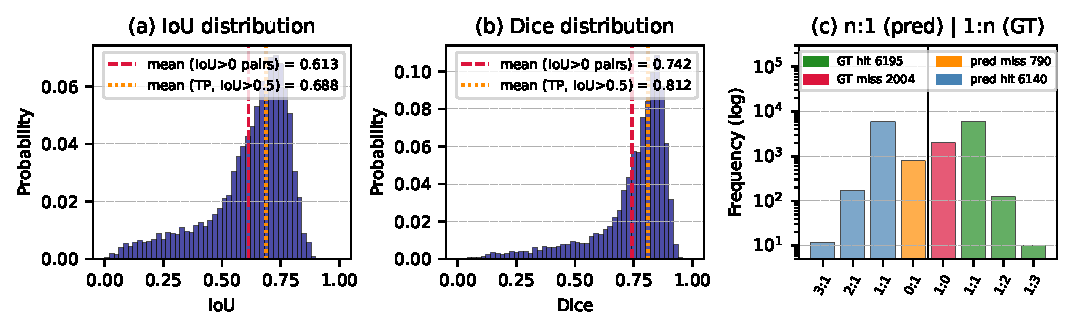
\includegraphics[width=\textwidth]{figures/host_plots.pdf}
\caption{Host self-evaluation plots for the V84 pipeline on 5-fold OOF predictions (707 training files, 8199
GT polygons over all records; PQ 0.4590 reproduced). Logic mirrors the host notebook
(\texttt{plot\_distribution}, \texttt{plot\_m2n\_counts}): all GT--prediction pairs with IoU$>$0 per annotator
record. (a) IoU, (b) Dice (=2IoU/(1+IoU) per pair), (c) number of overlapping partners per GT (1:$n$, right)
and per prediction (n:1, left).}
\label{fig:host}
\end{figure*}
Figure~\ref{fig:host} shows the three required distributions on OOF predictions. Over all overlapping pairs
the mean IoU is 0.613 (Dice 0.742); over matched pairs (IoU$>$0.5) 0.688 (Dice 0.812). The IoU mass sits at
0.65--0.80 and drops sharply above 0.85: annotators' own boundaries disagree at that level (human SQ
$\approx$0.63). Topology errors are rare: 134 of 8199 GT (1.6\%) overlap $\ge$2 predictions (fragmentation)
and 187 prediction-record pairs (2.7\%) overlap $\ge$2 GT (over-merging); 1:1 dominates on both sides. The
2004 GT with no overlapping prediction are mostly filaments drawn by a single annotator (below).

\section{Annotator-disagreement ceiling}
On the 296 multi-record training files we scored annotators against each other and computed label oracles
(all with access to GT, so they are ceilings, not achievable predictors):
\begin{itemize}
\item \textbf{Human vs.\ held-out human:} PQ \textbf{0.340} (SQ 0.634; 1196 ordered pairs). Our direct detector
scores 0.411 on the same records, so the model already beats a held-out annotator.
\item \textbf{Oracle predictors} (submit GT masks, scored against all records of the file): union of
annotators \textbf{0.663}; one annotator's own masks \textbf{0.605} (best/worst 0.631/0.571); majority/$k\ge2$
\textbf{0.592}; Dinkelbach-optimal subset of vote masks 0.668. Even perfect masks cap PQ near 0.6--0.67 because
records disagree on \emph{which} filaments exist.
\item \textbf{Keep-oracle:} choosing which of our own existing refined masks to keep using the true $q\cdot s$ gives
0.5283 (\textbf{+0.074}); our learned rule realises +0.003 of it, and a pixel-based quality head only +0.0019
more (Table~\ref{tab:post}). Agreement is weakly predictable from image or refiner evidence (Spearman with
true $q s$: 0.59 vs 0.57 for the score alone).
\item Recall on filaments drawn by $\ge$2 annotators is 0.834 vs 0.367 for single-annotator ones
(Fig.~\ref{fig:agree}a: 0.29 when one of three records drew it, 0.91 when all three did); fixing every
missed agreed filament would add only +0.030.
\item 764 of 1881 record-level FP (41\%) are filaments that another record of the same image drew
(Fig.~\ref{fig:agree}b); removing them would cost that record's TP.
\end{itemize}
\begin{figure}[t]\centering
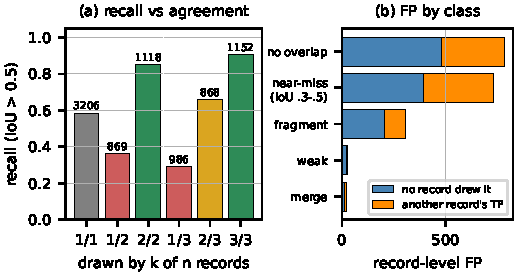
\includegraphics[width=\columnwidth]{figures/agreement.pdf}
\caption{V84 OOF errors vs annotator agreement (707 files). (a) Recall of annotated filaments by how many of
the image's $n$ records drew the same filament (polygons matched at IoU$>$0.5); bar labels are counts.
(b) Record-level FP by class (near-miss: best IoU 0.3--0.5; fragment: $\ge$50\% inside one GT), split by
whether another record of the same image drew the predicted filament.}
\label{fig:agree}
\end{figure}
The remaining gap is dominated by label disagreement, which no single-image model can resolve.

\section{Data use and rule compliance}
\begin{itemize}
\item \textbf{Training data:} only the provided training images and labels. No external ground truth of any
kind; no test labels or pseudo-labels on test images. Pretrained weights: COCO YOLO11s-seg (Ultralytics),
ImageNet ResNet18 (torchvision).
\item \textbf{Inference:} single-image; each test H$\alpha$ image alone (no neighbouring frames, no
magnetograms).
\item \textbf{Training-only experiments not in the final pipeline}, run under host rulings: (i) label transfer of
training polygons to nearby GONG frames $\pm$1--5 min, excluding any frame within $\pm$1 h of a test timestamp
(Kaggle discussion thread 748045); (ii) noisy-student pseudo-labelling on unlabelled GONG H$\alpha$ frames from
days excluding all train and test dates $\pm$1 day (thread 744047). Both were killed by their pre-registered
gates (Table~\ref{tab:neg}) and neither data source is used by the submitted models.
\end{itemize}

\section{Compute and efficiency}
Training on 4$\times$ NVIDIA T4 (one model per GPU; DDP is incompatible with the in-process stride-2 patch).
Final all-data detector: 2.4 h (stage 1, 80 ep) + 2.1 h (stage 2, 20 ep) = 4.5 GPU-h; all-data refiner 24 min;
LightGBM demote model: seconds on CPU. The full 5-fold OOF protocol costs $\approx$5$\times$ this.
\textbf{Inference:} 180 test images in 3 shards of 60 on one T4 each, 148--152 s per shard, i.e.
$\approx$\textbf{2.5 s/image} end-to-end (4-flip detector + 4-flip crop refiner + keep rule, model loading
included). A rerun from the repository on 2026-10-29 reproduced the submitted CSV byte-for-byte.

\section{Limitations}
The final gain over V65 (+0.005) is small and passed its gate narrowly; the all-data refiner and demote model
are single fits. Thin structures (barbs; agreed filaments narrower than 5 px: recall 0.60) remain the hardest morphology. The
largest open lever is predicting inter-annotator agreement (+0.074 keep-oracle headroom), which neither our
features nor a pixel-based quality head could reach (Fig.~\ref{fig:examples}).

\begin{figure}[t]\centering
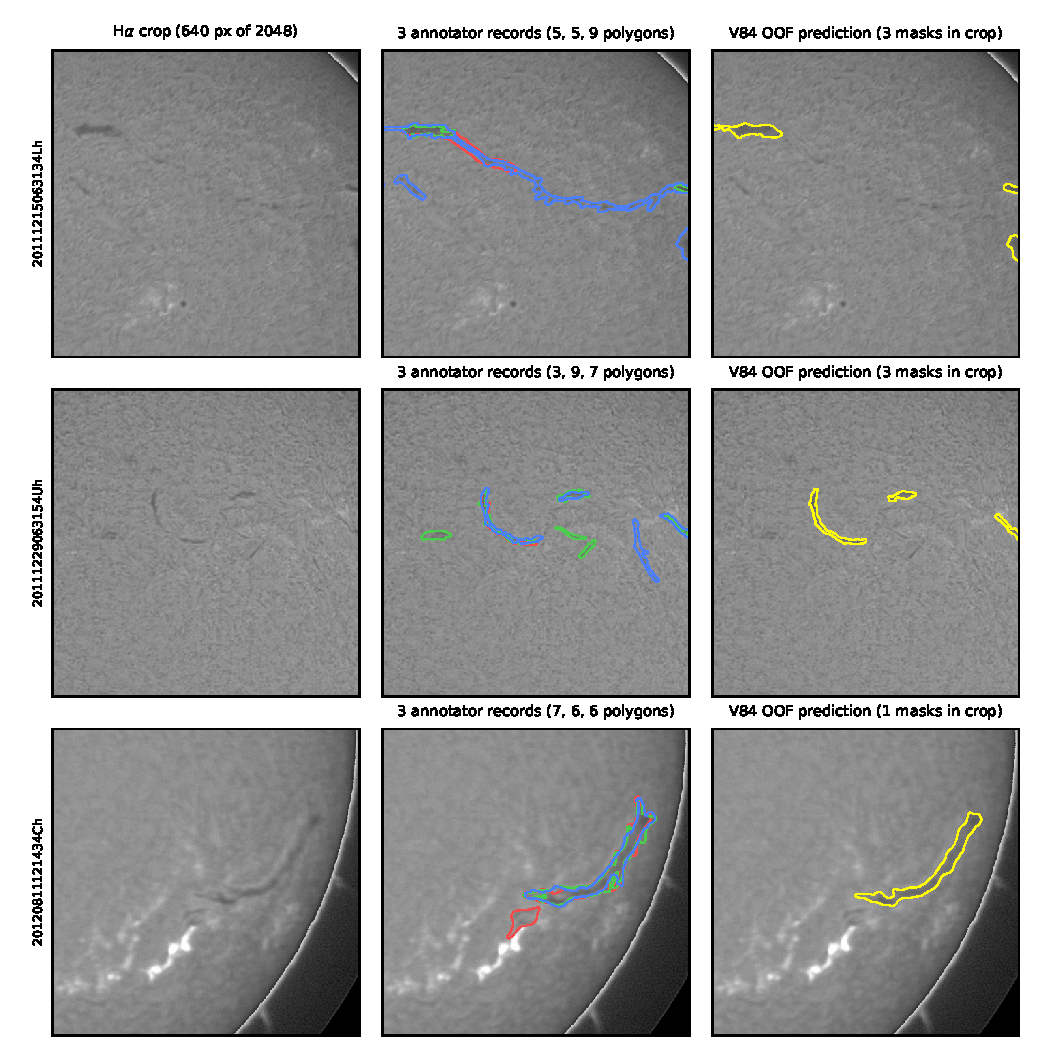
\includegraphics[width=\columnwidth]{figures/examples.pdf}
\caption{OOF examples, not chosen by score: the three 3-record training files with the median number of GT
polygons. Columns: H$\alpha$ crop (640 of 2048 px); the three annotator records (one colour each); V84
prediction from the model that did not see the file (yellow). Rows 2--3: filaments that all records drew are
found with matching extent, and most single-record polygons are left out, as the keep rule intends. Row 1: a
long, faint filament that one record draws whole and the other two only in parts is found only at its darkest
end, the most common kind of miss and one where the records themselves disagree on extent.}
\label{fig:examples}
\end{figure}

\end{document}
